% This is based on the LLNCS.DEM the demonstration file of
% the LaTeX macro package from Springer-Verlag
% for Lecture Notes in Computer Science,
% version 2.4 for LaTeX2e as of 16. April 2010
%
% See http://www.springer.com/computer/lncs/lncs+authors?SGWID=0-40209-0-0-0
% for the full guidelines.
%

\RequirePackage{amsmath}

\documentclass[runningheads,a4paper]{llncs}

\usepackage{amssymb}
\setcounter{tocdepth}{3}
\usepackage{graphicx}

%\usepackage{amsmath} % neprepisuji LLNCS symbol
\usepackage{amsfonts}
\usepackage[
backend=biber, 
style=numeric]{biblatex}
\usepackage[T1]{fontenc}
\usepackage[utf8]{inputenc}
\usepackage[caption=false]{subfig}
\usepackage{tikz}
\usepackage{url}
\usepackage{underscore}
\usepackage{pgffor}
\usepackage{pgfplots}
\usepackage{pgfplotstable}
\usepackage{newunicodechar}
\usepackage{algorithm}
\usepackage{algorithmic}
\usepackage{arrayjobx}
\usepackage{tikz}
\usepackage{textcomp}
\usepackage{xifthen}
\usepackage{mleftright}
\usepackage{enumitem}
\usepackage{fancyvrb}
\usepackage{float}
\usepackage{alltt}
\usepackage{hhline}
\usepackage{environ}
\usepackage{adjustbox}
\usepackage{mathtools}
\usepackage[short]{optidef}
\usepackage{longtable}
\usepackage{lscape}
\usepackage{makecell}
\usepackage{colortbl}
\usepackage{listings}
\usepackage{wrapfig}
\usepackage{hyperref}
\usepackage{booktabs}

\usepackage{url}
\urldef{\mailsa}\path|{martin.beseda, lubomir.riha, alexandros.markopoulos, petr.strakos}@vsb.cz|

\pgfplotsset{compat=1.14}

\DeclareFieldFormat{labelnumberwidth}{#1\adddot}
\setlength{\biblabelsep}{5pt}

\DeclareCaptionLabelFormat{andtable}{#1~#2  \&  \tablename~\thetable}

\addbibresource{bibliography.bib}
\addbibresource{statistics.bib}
\addbibresource{feti.bib}
\addbibresource{mpi.bib}
\addbibresource{directSolvers.bib}
\addbibresource{pardiso.bib}
\addbibresource{readex.bib}
\addbibresource{others.bib}
\newcommand*{\alert}{\textcolor{red}}

\makeatletter
% mynobreakpar
\newcommand\mynobreakpar{\par\nobreak\@afterheading} 
%
\renewcommand*\env@matrix[1][*\c@MaxMatrixCols c]{%
  \hskip -\arraycolsep
  \let\@ifnextchar\new@ifnextchar
  \array{#1}}
\makeatother

\allowdisplaybreaks

\lstset{
    literate={~} {$\sim$}{1}
}

\begin{document}

\title{Performance Modeling of the HTFETI Solver Implementation in the ESPRESO Library}
%
\titlerunning{Performance Modeling the HTFETI Solver}  % abbreviated title (for running head)
%                                     also used for the TOC unless
%                                     \toctitle is used
%
\author{Martin Beseda\inst{a} \and Lubom\'{i}r \v{R}\'{i}ha\inst{a} \and Alexandros Markopoulos\inst{a} \and Petr Strako\v{s}\inst{a}}
%
\authorrunning{Performance Modeling the HTFETI Solver} % abbreviated author list (for running head)
%
%%%% list of authors for the TOC (use if author list has to be modified)
%\tocauthor{Ivar Ekeland, Roger Temam, Jeffrey Dean, David Grove,
%Craig Chambers, Kim B. Bruce, and Elisa Bertino}
%
\institute{$^a$IT4Innovations National Supercomputing Centre, VSB-Technical University of Ostrava, Ostrava, Czech Republic\\
%\email{martin.beseda@vsb.cz, lubomir.riha@vsb.cz, alexandros.markopoulos@vsb.cz}
\mailsa\\
\texttt{http://www.it4i.cz}
}
%\\ WWW home page:
%\texttt{http://users/\homedir iekeland/web/welcome.html}
%\and
%Universit\'{e} de Paris-Sud,
%Laboratoire d'Analyse Num\'{e}rique, B\^{a}timent 425,\\
%F-91405 Orsay Cedex, France}

\maketitle              % typeset the title of the contribution

\begin{abstract}

The main objective of this paper is the development and implementation of the 
performance model for prediction of the runtime of the 
Total FETI and Hybrid Total FETI methods implemented in the ESPRESO library.

The final performance model consists of several partial ones, each created by 
a generalized linear regression, using R-language. These models were created from 
set of calibration measurements.

The final performance model is designed for prediction of the optimal settings 
of the solvers in a sense of optimal domain decomposition and optimal number of 
MPI processes and OpenMP threads. The user only provides the size of the problem 
to be solved.

Our tests show that the final model can predict optimal settings with an error 
smaller than 1s for a solver runtime that can vary between 3 and 50 seconds 
based on problem decomposition and parallelization setup.  

\keywords{performance model, ESPRESO, FETI, MPI, OpenMP}
\end{abstract}
%

\section{Motivation}
The motivation for the work presented in this paper is a fact that there exist several 
implementations of various FETI methods but it is very difficult for their users to 
setup them efficiently to minimize the runtime of the solver and to efficiently utilize the 
given hardware. 

Therefore this paper proposes a performance model for a massively parallel implementation of 
the Total FETI (TFETI) and Hybrid Total FETI (HTFETI) solvers in the 
ESPRESO library \cite{vriha2016massively}.


This model allows any inexperienced user to set-up both solvers in sense of 
(1) optimal domain decomposition and 
(2) optimal OpenMP and MPI parallelization, 
to minimize the solver runtime. 
Our model takes into account the parallel scalability of the solver however 
it is not able to predict the numerical scalability. In other words, model determines the minimal single iteration time, but it cannot predict how many iterations is needed 
to solve the problem because it is highly problem dependent.  


The model is composed of several partial models. Each of these estimates the run-time of a separate region. This enables easier customization of the model for future 
versions of ESPRESO as well as more detailed information of the solver behavior for 
different settings. 



\section{FETI Methods}
The FETI (Finite Element Tearing and Interconnecting) method was introduced by Farhat and Roux 
in \cite{feti1}. It is the method used to solve linear problem described by elliptic PDEs in 
parallel. It decomposes the spatial domain into non-overlapping sub-domains "glued" together 
by Lagrange multipliers. The primal problem is then transferred, or rather reduced, into the 
smaller and better conditioned constrained QP problem. This problem is then solved iteratively,
typically using some form of Conjugate Gradient (CG) method.


The FETI method was modified (described in \cite{feti1optimal}), when it was observed, that the mathematical 
treatment of floating sub-domains together with the Projected Conjugate Gradients method 
(described in \cite{vriha2016massively} in detail) is equivalent to the assembling and solution 
of a coarse problem, which accelerates the convergence and guarantees, that the FETI algorithm 
numerical  performance is independent on a number of sub-domains.

For practical purposes a method for automatic identification of kernels of the
subdomain stiffness matrices is required. These kernels are used during the elimination of the primal 
variables and in definition of the coarse grid projectors. The algorithm for kernel detection was
described by Farhat and Gérardin in \cite{feti1optimal2} as the combination of Cholesky 
factorization and the singular value decomposition.

The kernel detection problem partially persisted in real-world problems even with this 
improvement, because of the rounding errors. This led to the improved version of FETI called 
FETI-DP described in \cite{fetidp}. The difference is, that FETI-DP makes all the subdomain stiffness
matrices invertible by enforcing the continuity of displacements at the corners 
on primal level. This is advantageous for some applications, because FETI-DP is efficiently 
preconditioned and so it converges better than FETI. The main drawback is, that the coarse grid
defined by the corners is less efficient without additional preconditioning than the one defined
by the rigid body motions, as described in \cite{fetidpDostal}. The FETI-DP algorithm is also 
much more difficult to implement, because it requires a special treatment of corners. The algorithm, which addresses both of these drawbacks is called Total FETI (TFETI) and it is briefly introduced in the next section. % (described in detail in TODO).


\subsection{Total FETI}
After discretization and decomposition into sub-domains, the i-th
sub-domain corresponds to the following system: 

\begin{align}
K_i u_i &= f_i - B_i^T \lambda, \qquad i \in \{ 1, \ldots, n \}\\
B_i u_i &= c_i,
\label{eq:tfetiLocalProblem}
\end{align}
where $K_i$ is the local stiffness matrix of the i-th sub-domain, 
$f_i$ is the local right-hand side vector, $B_i$ is the constraint matrix and $n$ is the number of 
sub-domains. Finally, $\lambda$ is a vector of Lagrange 
multipliers, which enforces the continuity of neighboring 
sub-domains.


Moreover, the problem is accompanied by the compatibility 
condition
\begin{equation}
B_1 u_1 + \cdots + B_n u_n = c,
\end{equation}
where $c \in \mathbb{R}$. $B_i$ matrices can be assembled into 
a global matrix $B = \left[ B_1, \ldots, B_n \right]$, which enforces both the Dirichlet boundary conditions and the continuity of neighboring sub-domains.% in the decomposed  problem.

One can also assemble the global stiffness matrix $K = diag\left( K_1, \ldots, K_n \right)$, the global right-hand side vector $f = \left[ f_1^T, \ldots, f_n^T \right]^T$ and the global unknown vector $u = \left[ u_1^T, \ldots, u_n^T \right]^T$,
so the whole problem can be rewritten as 
\begin{equation}
\begin{bmatrix}
K & B^T\\
B & O
\end{bmatrix}
\begin{bmatrix}
u\\
\lambda
\end{bmatrix}
=
\begin{bmatrix}
f\\
c
\end{bmatrix}.
\label{eq:tfetiGlobProb}
\end{equation}
By eliminating primary variable $u$ as 
\begin{equation}
u = K^\dagger \left( f - B^T \lambda \right) + R\alpha
\label{eq:elimUVar}
\end{equation}
and by utilizing orthogonality condition 
\begin{equation}
R \perp f - B^T \lambda
\label{eq:tfetiOrthogCond}
\end{equation}
we get a new system with a Schur complement
\begin{equation}
\begin{bmatrix}
F & G \\
G^T & O
\end{bmatrix}
\begin{bmatrix}
\lambda\\
\alpha
\end{bmatrix}
=
\begin{bmatrix}
d\\
e
\end{bmatrix},
\label{eq:tfetiDualProblem}
\end{equation}
where 
\begin{align}
F &= BK^\dagger B^T\\
G &= -BR\\
d &= BK^\dagger f - c\\
e &= -R^T f^T,\end{align}
and $R = diag\left( R_1, \ldots, R_n \right)$ consisting of the vectors which create the a basis of the null space of the matrix $K$.
The new system given by Eq. \eqref{eq:tfetiDualProblem} is smaller and better conditioned, than the original problem, so it can be solved more efficiently. To solve the system the Projected Preconditioned Conjugate Gradient (PPCG) method is used. This method is using the projector 
\begin{equation}
P = I - G\left( G^T G \right)^{-1} G^T,
\end{equation}
where $G = -BR$. Size of the so called \textit{coarse problem} $G^T G \in \mathbb{R}^{n_G \times n_G}$ depends on the number of sub-domains $n$, such as
$n_G = n \cdot d$, where $d$ is the number of rigid body motions (3 in 2D, 6 in 3D for linear elasticity problem). The coarse problem could become a bottle-neck of TFETI algorithm when solving very large problems. This problem is addressed by HTFETI method.


\subsection{Hybrid Total FETI }
The key idea of HTFETI is the aggregation of a  
number of neighboring sub-domains into so called 
\textit{clusters} using Lagrange multipliers, which results 
into a smaller coarse problem. Using Lagrange multipliers here means, that the TFETI method is used twice - both on cluster and sub-domain levels.


So, the problem is decomposed into $n = n_c \cdot n_s$ sub-domains 
in total, $n_c$ being the number of clusters and $n_s$ being the number of sub-domains per cluster.


In HTFETI there is used slightly modified form of the problem described as
\begin{mini}
    {u}{\frac{1}{2}u^T K u - u^T f}{}{}
    \addConstraint{B_0u = c_0}
    \addConstraint{B_1u = c_1}
    \label{eq:htfetiProblem}
\end{mini}
The first part $B_0 u = c_0$ of the equality constraints enforces
the continuity in the sub-domain corner nodes of each cluster and the second part $B_1 u = c_1$ enforces the continuity among the rest of the sub-domain interfaces
and the prescribed Dirichlet condition.


The problem \eqref{eq:htfetiProblem} can be described with respect to the Karush-Kuhn-Tucker conditions as
\begin{equation}
\begin{bmatrix}[cc|c]
K & B_0^T & B_0^T \\
B_0 & O & O \\ \hline
B_1 & O & O
\end{bmatrix}
\begin{bmatrix}
u\\
\lambda_0\\ \hline
\lambda_1
\end{bmatrix}
=
\begin{bmatrix}
f\\
c_0\\ \hline
c_1
\end{bmatrix}.
\label{eq:htfetiProblemModif1}
\end{equation}
This equation can be rewritten further as
\begin{equation}
\begin{bmatrix}[c|c]
\tilde{K} & \tilde{B}^T\\ \hline
\tilde{B} & O
\end{bmatrix}
\begin{bmatrix}
\tilde{u}\\
\tilde{\lambda}
\end{bmatrix}
=
\begin{bmatrix}
\tilde{f}\\
\tilde{c}
\end{bmatrix},
\label{eq:htfetiProblemModif2}
\end{equation}
The Schur complement can be derived from Eq. 
\eqref{eq:htfetiProblemModif2} using steps like in 
Eq. \eqref{eq:tfetiGlobProb}, \eqref{eq:elimUVar}, 
\eqref{eq:tfetiOrthogCond} and 
\eqref{eq:tfetiDualProblem}, so we get the new 
problem
\begin{equation}
\left[
\begin{array}{lr}
\tilde{F} & \tilde{G} \\
\tilde{G}^T & O
\end{array}
\right]
\begin{bmatrix}
\tilde{\lambda}\\
\tilde{\alpha}
\end{bmatrix}
=
\begin{bmatrix}
\tilde{d}\\
\tilde{e}
\end{bmatrix},
\label{eq:htfetiDualProblem}
\end{equation}
which is easily solvable than the original problem, because the coarse problem $\tilde{G}^T\tilde{G} \in \mathbb{R}^{n_G \times n_G}$ is significantly smaller. Its size depends on the number of clusters and not sub-domains like
\begin{equation}
n_{\tilde{G}} = \left(\# \, clusters\right) \times \left(\# \, RBM \right).
\end{equation}
This new problem can be also solved by PPCG algorithm in the same way as \eqref{eq:tfetiDualProblem}.

%\section{Performance Modeling of the FETI Solvers }

In this section we describe the NUMA effects which significantly affects the performance model, the benchmark problem used for calibration of the model, the approach used for creating the partial models for different blocks of the TFETI and HTFETI solvers and the assembling process of the full model. 

\subsection{NUMA Effect}
\label{sec:numa}
% Processors with architecture Haswell-EP used in Salomon supercomputer (see description in Sec. 
% \ref{sec:salomonDescription}) have 12-core dies. It is designed as it is depicted in Fig. 
% \ref{fig:haswellSocket}, i.e. there are two bi-directional rings in one die. Eight cores with 
% respective slices of L3 cache, QPI interconnect, a memory controller and the PCIe controller are 
% connected to the first ring.


% The remaining four cores with their respective L3 cache slices and the second memory controller 
% are connected to the second bi-directional ring. The rings are then connected together by two 
% queues. Threads from every core can access all DDR4 memory units. It is clear that accessing the local memory, in this case memory on the 
% local ring, is faster, than accessing the remote one (using the memory controller on remote 
% ring). This, so called, \textit{Non-Uniform Memory Access (NUMA)} effect can significantly affect 
% the behavior of parallel applications. 


% This leads us to two types of a possible delay caused by accessing remote memory units. Both types of
% delay are usually called \textit{NUMA effect} and the first type is caused by reading from RAM memory 
% connected closely to the other ring, e.g. accessing DDR4 D memory by thread bounded to the Core 3, 
% considering the Fig. \ref{fig:haswellSocket}. The delay is caused by data transfer through some of the
% queues between the two bi-directional rings.


\begin{figure}[!thb]
\centering
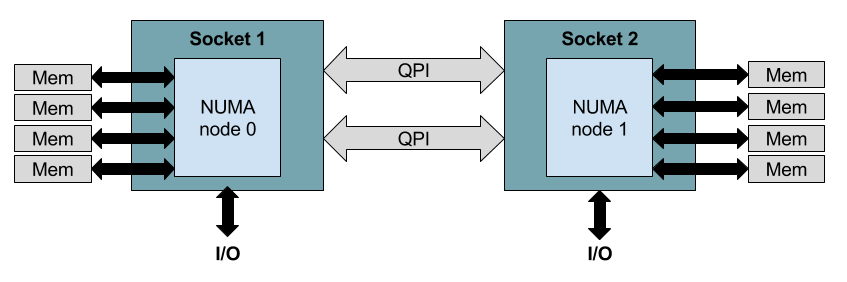
\includegraphics[scale=0.4]{figures/numa.png}
\caption{Dual socket Xeon E5 v3 system - one NUMA node per socket (source \cite{molka2015cache})}
\label{fig:haswellDualSocket}
\end{figure}


%The second and the more significant type of 
The most notable version of the NUMA effect in today HPC clusters is caused by accessing memory attached to another 
socket (i.e.processor) in a multi CPU/socket system. As can be seen from the Fig. \ref{fig:haswellDualSocket}, 
data have to be transferred through the QPI link which decreases the bandwidth and increase the latency of memory transfers. More details about the memory subsystem of the Haswell Xeon CPU can be found in \cite{molka2015cache}.

\section{Performance Modeling of the FETI Solvers }
\subsection{Benchmark Problem}
The computed problem is generated by \textit{Parallel Problem Generator (PPG)}. PPG is a part of the ESPRESO library and it is designed to enable fast evaluation of the solver for 
very large problems of linear elasticity (described in \cite{vriha2016massively}). 
It generates a benchmark problems in form of the 
steel cube with following properties: 
Volume $V = 9000\,mm^3$,  
Elastic modulus $E = 2.1 \cdot 10^5\,MPa$,  
Poisson's ratio $\mu = 0.3$,  
Density $\rho = 7850 kg\,m^{-3}$, 
Gravity constant $g = 9.81 m\,s^{-1}$.
The cube is loaded with its own weight in the $x$ direction and 
it is fixed on the plane $x = 0$.

The discretization process consists of two steps: (1) generating cubical meshes (
one per each cluster); and (2) decomposition of the cluster meshes into cubical sub-
domains using geometric decomposition (METIS based decomposition is also supported). 
For this paper all discretization is done using 8-node brick elements.


% The matrix assembler then creates following objects according to the mesh data:

% \begin{itemize}
% 	\item Stiffness matrix $K_i$
% 	\item RHS $f_i$
% 	\item "Gluing" matrix $B_i$
% 	\item Matrix of HTFETI corners $B_{0,i}$
% 	\item Set of fixed nodes used for regularization of $K_i$ in TFETI (described in \cite{brzobohaty2011cholesky})
% \end{itemize}

%\begin{wrapfigure}[13]{R}{0.4\textwidth}
\begin{figure}
\centering
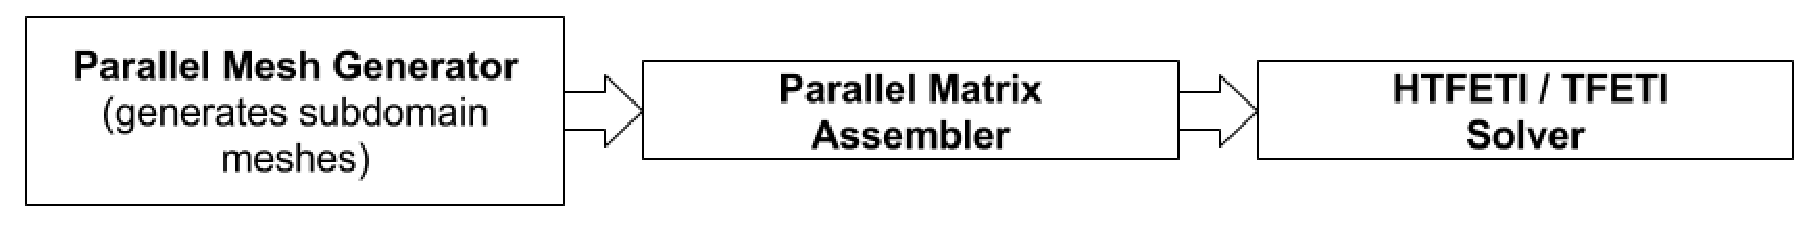
\includegraphics[scale=0.4]{figures/meshGen.pdf}
\caption{\label{fig:espresoMeshInp} ESPRESO benchmark generator and solver diagram (source \cite{vriha2016massively})}
\end{figure}

% $K_i$ and $f_i$ are created in parallel, using multiple Cilk++ 
% threads. The matrix $B_i$ is assembled from 3 parts:

% \begin{itemize}
% 	\item Dirichlet boundary conditions
% 	\item "Gluing" among sub-domains (i.e. inside cluster)
% 	\item "Gluing" among clusters
% \end{itemize}

% Dirichlet boundary conditions and "gluing" among sub-domains are independent among clusters and
% row indices are globally renumbered after they are assembled on all clusters. Renumbering is 
% performed by single call of \texttt{MPI\_Scan()}\cite{mpiScan} function.

% Assembling the third part, which arranges "gluing" among clusters employs the nearest-neighbor 
% strategy - it performs an exchange of global indices of surface DOF among the neighboring 
% clusters. It is performed in parallel among clusters and its most time consuming 
% operations, like binary search in an array for every surface DOF, can be further parallelized
% by threads.

\subsection{Modeling Approach for Partial Models}

The full model is assembled from several partial models, which cover the most 
significant, i.e. time-demanding, regions of the ESPRESO solver. The partials models take
number of nodes \verb!nnodes!, number of processes per node \verb!nprocs!,
number of domains per node \verb!ndoms! and number of DOF per MPI process \verb!nDOF!
as inputs.

The partial models were created by generalized linear regression with natural logarithm as a link function to enforce positive values of the output variable (i.e. time). This was performed using R-language \cite{rDocs}
%, which is very briefly described in Appendix \ref{sec:r}.

In the rest of this section the modeling approach is explained on partial model describing the action of the stiffness matrix $K$ in HTFETI. The application of the HTFETI $\tilde{F}$-operator (which is not assembled explicitly in ESPRESO) is show in Eq. \eqref{eq:htfetiDualProblem}. 

The modeling itself is an iterative process. The first version of the model is shown in the Eq. \eqref{eq:actionKHTFETIFull}, containing 
polynomial of every predictor variable and all their interactions, so we do not omit anything. The variable $nprocs$ is described as a fraction $\frac{1}{nprocs}$, because data which depends on it lies on a hyperbola, which is caused by a significant NUMA effect (as described in \cite{molka2015cache}).


\begin{equation}
\label{eq:actionKHTFETIFull}
\begin{aligned}
t_{K|act|HT} \sim\; &\mathrm{(poly(I(1/nprocs), 2) + poly(ndoms, 2)}\\
&+ \mathrm{poly(nDOF, 2))\,\widehat{}\,3}
\end{aligned}
\end{equation}
The summary of the model (see Tab. \ref{tab:actionKHTFETI}) shows, that only some of the main effects  significantly contribute to the model. The proposed model fits much better then the null model, as can be seen from listed deviances. 
Also we can see, that Fisher scoring algorithm (described in \cite{fischerScoringAlg}), 
found some optima, because there is the finite number of its iterations.


\begin{table}[!hptb]
\centering
\scriptsize
%\resizebox{\textwidth}{!}{
\begin{tabular}{llllll}
 & \textbf{t value} & \textbf{Pr(\textgreater|t|)} & \textbf{} \\
\textbf{(Intercept)} & -85.758 & \textless 2e-16 & *** \\
\textbf{poly(I(1/nprocs), 2)1} & 1.244 & 0.21546 &  \\
\textbf{poly(I(1/nprocs), 2)2} & -0.188 & 0.85098 &  \\
\textbf{poly(ndoms, 2)1} & 21.908 & \textless 2e-16 & *** \\
\textbf{poly(ndoms, 2)2} & -3.227 & 0.00155 & ** \\
\textbf{poly(nDOF, 2)1} & 47.715 & \textless 2e-16 & *** \\
\textbf{poly(nDOF, 2)2} & -19.592 & \textless 2e-16 & *** \\
\textbf{poly(I(1/nprocs), 2)1:poly(ndoms, 2)1} & 0.036 & 0.97125 &  \\
\textbf{\vdots} & \vdots & \vdots &  \\
\textbf{poly(I(1/nprocs), 2)1:poly(ndoms, 2)1:poly(nDOF, 2)1} & -0.045 & 0.96445 &  \\
\textbf{\vdots} & \vdots & \vdots &  \\
\hhline{====}
\textbf{Null deviance} & \multicolumn{1}{r}{9.766522 (167DOF)} &  &  \\
\textbf{Residual deviance} & \multicolumn{1}{r}{0.030749 (141DOF)} &  &  \\
\textbf{AIC} & \multicolumn{1}{r}{-913.02} &  &  \\
\textbf{Fisher Scoring it.} & \multicolumn{1}{r}{6} &  & 
\end{tabular}
%}
\caption{Action of $K$ - HTFETI (1st model)}
\label{tab:actionKHTFETI}
\vspace{1.5em}
\scriptsize
%\resizebox{\textwidth}{!}{
\begin{tabular}{llllll}
 & \textbf{Estimate} & \textbf{Std. Error} & \textbf{t value} & \textbf{Pr(\textgreater|t|)} &  \\
\textbf{(Intercept)} & -2.63321 & 0.01217 & -216.33 & \textless 2e-16 & *** \\
\textbf{I(1/nprocs)} & 0.05772 & 0.01081 & 5.34 & 3.14e-07 & *** \\
\textbf{poly(ndoms, 3)1} & 6.70538 & 0.02693 & 248.99 & \textless 2e-16 & *** \\
\textbf{poly(ndoms, 3)2} & -1.18015 & 0.03270 & -36.09 & \textless 2e-16 & *** \\
\textbf{poly(ndoms, 3)3} & 0.15667 & 0.03775 & 4.15 & 5.38e-05 & *** \\
\textbf{poly(nDOF, 3)1} & 16.45273 & 0.13900 & 118.37 & \textless 2e-16 & *** \\
\textbf{poly(nDOF, 3)2} & -4.97680 & 0.10190 & -48.84 & \textless 2e-16 & *** \\
\textbf{poly(nDOF, 3)3} & 1.30552 & 0.05489 & 23.79 & \textless 2e-16 & *** \\
\hhline{======}
\textbf{Null deviance} & \multicolumn{1}{r}{9.7665223  (167 DOF)} &  &  &  &  \\
\textbf{Residual deviance} & \multicolumn{1}{r}{0.0056578 (160 DOF)} &  &  &  &  \\
\textbf{AIC} & \multicolumn{1}{r}{-1235.4} &  &  &  &  \\
\textbf{Fisher Scoring it.} & \multicolumn{1}{r}{5} &  &  &  & 
\end{tabular}
%}
\caption{Action of $K$ - HTFETI (improved model)}
\label{tab:actionKHTFETIimp}
\vspace{1.5em}
\scriptsize
%\resizebox{\textwidth}{!}{
\begin{tabular}{llllll}
\multicolumn{1}{c}{} & \textbf{Estimate} & \textbf{Std. Error} & \textbf{t value} & \textbf{Pr(\textgreater|t|)} & \multicolumn{1}{c}{} \\
\textbf{(Intercept)} & -6.693e+00 & 1.168e-01 & -57.284 & \textless 2e-16 & *** \\
\textbf{I(1/nprocs)} & 5.772e-02 & 1.081e-02 & 5.340 & 3.14e-07 & *** \\
\textbf{poly(ndoms, 3, raw = T)1} & 6.047e-03 & 6.210e-04 & 9.738 & \textless 2e-16 & *** \\
\textbf{poly(ndoms, 3, raw = T)2} & -5.647e-06 & 1.046e-06 & -5.398 & 2.39e-07 & *** \\
\textbf{poly(ndoms, 3, raw = T)3} & 2.126e-09 & 5.123e-10 & 4.150 & 5.38e-05 & *** \\
\textbf{poly(nDOF, 3, raw = T)1} & 7.290e-04 & 1.524e-05 & 47.847 & \textless 2e-16 & *** \\
\textbf{poly(nDOF, 3, raw = T)2} & -5.256e-08 & 1.759e-09 & -29.874 & \textless 2e-16 & *** \\
\textbf{poly(nDOF, 3, raw = T)3} & 1.473e-12 & 6.193e-14 & 23.785 & \textless 2e-16 & *** \\ \hhline{======}
\textbf{Null deviance} & \multicolumn{1}{r}{9.7665223 (167 DOF)} &  &  &  &  \\
\textbf{Residual deviance} & \multicolumn{1}{r}{0.0056578 (160 DOF)} &  &  &  &  \\
\textbf{AIC} & \multicolumn{1}{r}{-1235.4} &  &  &  &  \\
\textbf{Fisher Scoring it.} & \multicolumn{1}{r}{5} &  &  &  & \\
\hhline{======}
\multicolumn{2}{c}{\textbf{Cross-validation}} &  &  &  &  \\
\textbf{mean(RMSE)} & \multicolumn{1}{r}{0.005745} &  &  &  &  \\
\textbf{sd(RMSE)} & \multicolumn{1}{r}{0.001180} &  &  &  &  \\
\textbf{mean(MAPE)} & \multicolumn{1}{r}{0.158468} &  &  &  &  \\
\textbf{sd(MAPE)} & \multicolumn{1}{r}{0.037536} &  &  &  &
\end{tabular}
%}
\caption{Action of $K$ - HTFETI (final model)}
\label{tab:actionKHTFETIFinal}
\end{table}


So, in the next step we will remove all the interactions and the quadratic term of the $nprocs$ 
polynomial, because, as we can see in the summary, it is marked as non-significant too. 
The linear term of this polynomial has also high p-value, but it is not convenient to remove all the main effects of some predictor variable just because of the Wald test. The reason is that after removing 
some terms the remaining ones can be already detected as significant ones. And even if the 
remaining main effects would not be detected as significant by the Wald test, the model has usually 
better predictive capability with the main effects included for all predictor variables.


The new model is described as
\begin{equation}
\label{eq:actionKHTFETIimp}
t_{K|act|HT} \sim\; \mathrm{I(1/nprocs) + poly(ndoms, 3) + poly(nDOF, 3)\,.}
\end{equation}
As we can see in the Tab. \ref{tab:actionKHTFETIimp}, all the terms in the model are now detected as significant by Wald test. Akaike information criterion (AIC) is much lower than previous -913.02, which denotes the significant
improvement of the model. Moreover the residual deviance is significantly lower than the null deviance, which means great improvement over the null model, i.e. the well-fitting model on the data-set.

% \begin{table}[H]
% \centering
% \resizebox{\textwidth}{!}{
% \begin{tabular}{llllll}
%  & \textbf{Estimate} & \textbf{Std. Error} & \textbf{t value} & \textbf{Pr(\textgreater|t|)} &  \\
% \textbf{(Intercept)} & -2.63321 & 0.01217 & -216.33 & \textless 2e-16 & *** \\
% \textbf{I(1/nprocs)} & 0.05772 & 0.01081 & 5.34 & 3.14e-07 & *** \\
% \textbf{poly(ndoms, 3)1} & 6.70538 & 0.02693 & 248.99 & \textless 2e-16 & *** \\
% \textbf{poly(ndoms, 3)2} & -1.18015 & 0.03270 & -36.09 & \textless 2e-16 & *** \\
% \textbf{poly(ndoms, 3)3} & 0.15667 & 0.03775 & 4.15 & 5.38e-05 & *** \\
% \textbf{poly(nDOF, 3)1} & 16.45273 & 0.13900 & 118.37 & \textless 2e-16 & *** \\
% \textbf{poly(nDOF, 3)2} & -4.97680 & 0.10190 & -48.84 & \textless 2e-16 & *** \\
% \textbf{poly(nDOF, 3)3} & 1.30552 & 0.05489 & 23.79 & \textless 2e-16 & *** \\
% \hhline{======}
% \textbf{Null deviance} & \multicolumn{1}{r}{9.7665223  (167 DOF)} &  &  &  &  \\
% \textbf{Residual deviance} & \multicolumn{1}{r}{0.0056578 (160 DOF)} &  &  &  &  \\
% \textbf{AIC} & \multicolumn{1}{r}{-1235.4} &  &  &  &  \\
% \textbf{Fisher Scoring it.} & \multicolumn{1}{r}{5} &  &  &  & 
% \end{tabular}
% }
% \caption{Action of $K$ - HTFETI (improved model)}
% \label{tab:actionKHTFETIimp}
% \end{table}

So, we can change the model to use ordinary polynomials as 

\begin{equation}
\label{eq:actionKHTFETIFfinal}
\begin{aligned}
t_{K|act|HT} \sim\; &\mathrm{I(1/nprocs) + poly(ndoms, 3, raw=T)}\\
&+ \mathrm{poly(nDOF, 3, raw=T)}
\end{aligned}
\end{equation}
and perform cross-validation to evaluate the predictive capability of the model. The estimated coefficients are listed in Tab. \ref{tab:actionKHTFETIFinal}.

% \begin{table}[H]
% \centering
% \resizebox{\textwidth}{!}{
% \begin{tabular}{llllll}
% \multicolumn{1}{c}{} & \textbf{Estimate} & \textbf{Std. Error} & \textbf{t value} & \textbf{Pr(\textgreater|t|)} & \multicolumn{1}{c}{} \\
% \textbf{(Intercept)} & -6.693e+00 & 1.168e-01 & -57.284 & \textless 2e-16 & *** \\
% \textbf{I(1/nprocs)} & 5.772e-02 & 1.081e-02 & 5.340 & 3.14e-07 & *** \\
% \textbf{poly(ndoms, 3, raw = T)1} & 6.047e-03 & 6.210e-04 & 9.738 & \textless 2e-16 & *** \\
% \textbf{poly(ndoms, 3, raw = T)2} & -5.647e-06 & 1.046e-06 & -5.398 & 2.39e-07 & *** \\
% \textbf{poly(ndoms, 3, raw = T)3} & 2.126e-09 & 5.123e-10 & 4.150 & 5.38e-05 & *** \\
% \textbf{poly(nDOF, 3, raw = T)1} & 7.290e-04 & 1.524e-05 & 47.847 & \textless 2e-16 & *** \\
% \textbf{poly(nDOF, 3, raw = T)2} & -5.256e-08 & 1.759e-09 & -29.874 & \textless 2e-16 & *** \\
% \textbf{poly(nDOF, 3, raw = T)3} & 1.473e-12 & 6.193e-14 & 23.785 & \textless 2e-16 & *** \\ \hhline{======}
% \textbf{Null deviance} & \multicolumn{1}{r}{9.7665223 (167 DOF)} &  &  &  &  \\
% \textbf{Residual deviance} & \multicolumn{1}{r}{0.0056578 (160 DOF)} &  &  &  &  \\
% \textbf{AIC} & \multicolumn{1}{r}{-1235.4} &  &  &  &  \\
% \textbf{Fisher Scoring it.} & \multicolumn{1}{r}{5} &  &  &  & \\
% \hhline{======}
% \multicolumn{2}{c}{\textbf{Cross-validation}} &  &  &  &  \\
% \textbf{mean(RMSE)} & \multicolumn{1}{r}{0.005745} &  &  &  &  \\
% \textbf{sd(RMSE)} & \multicolumn{1}{r}{0.001180} &  &  &  &  \\
% \textbf{mean(MAPE)} & \multicolumn{1}{r}{0.158468} &  &  &  &  \\
% \textbf{sd(MAPE)} & \multicolumn{1}{r}{0.037536} &  &  &  &
% \end{tabular}
% }
% \caption{Action of $K$ - HTFETI (final model)}
% \label{tab:actionKHTFETIFinal}
% \end{table}


As we can see, the coefficients differ dramatically from the previous 
ones, but all the terms significantly contribute to the model. Predicted
values did not change, as we can see from the null deviance, residual
deviance and AIC being the same. We can see the visualized fit on the all 
data-set used for training in Fig. \ref{fig:actionK-HTFETI}. There were performed 15 iterations of repeated random sub-sampling cross-validation. The results are 
listed in the Tab. 
\ref{tab:actionKHTFETIFinal}.
% and visualized in Fig. \ref{fig:actionK-HTFETI-crossVal}.
As we can see, expected values of RMSE and MAPE are pretty low and their 
standard deviations are low too. Therefore the predictive capability of this
model is good and it does not tend to worsen significantly for some 
training sets.


\begin{figure}[htb]
\centering
%\adjustbox{max width=\linewidth}{
%\begin{minipage}{0.6\linewidth}
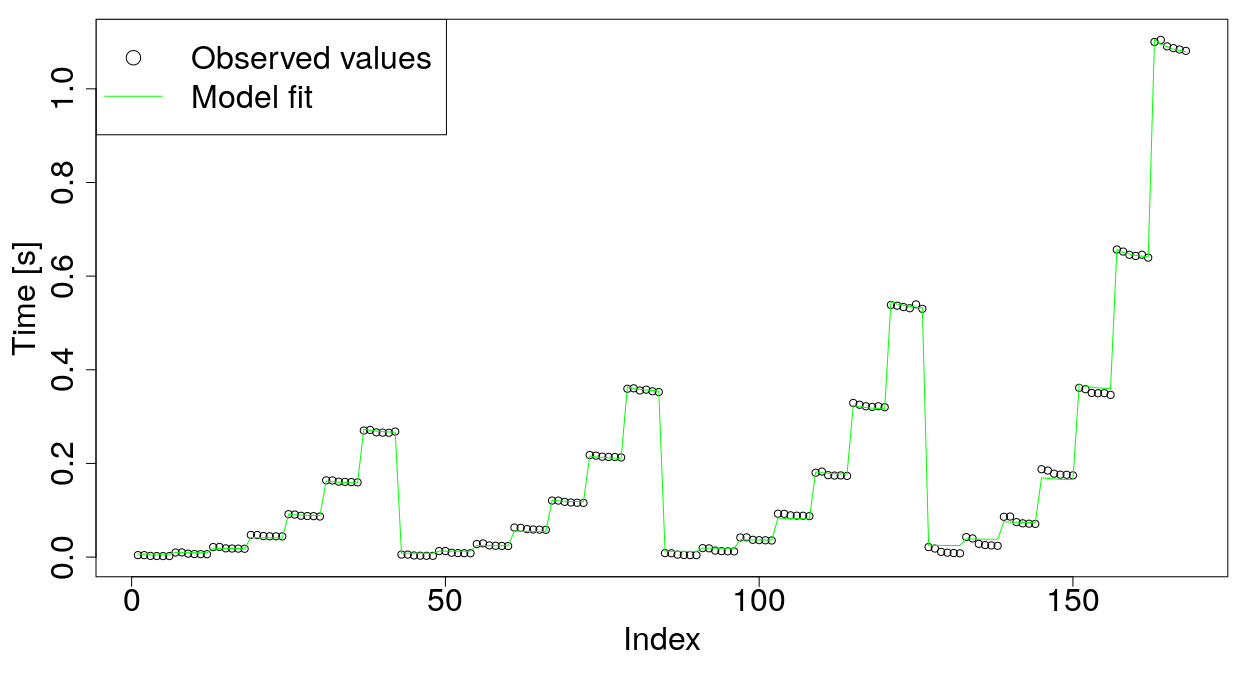
\includegraphics[scale=0.22]{figures/actionK-HTFETI.png}
%\end{minipage}
%\hfill
%\begin{minipage}{0.3\linewidth}
%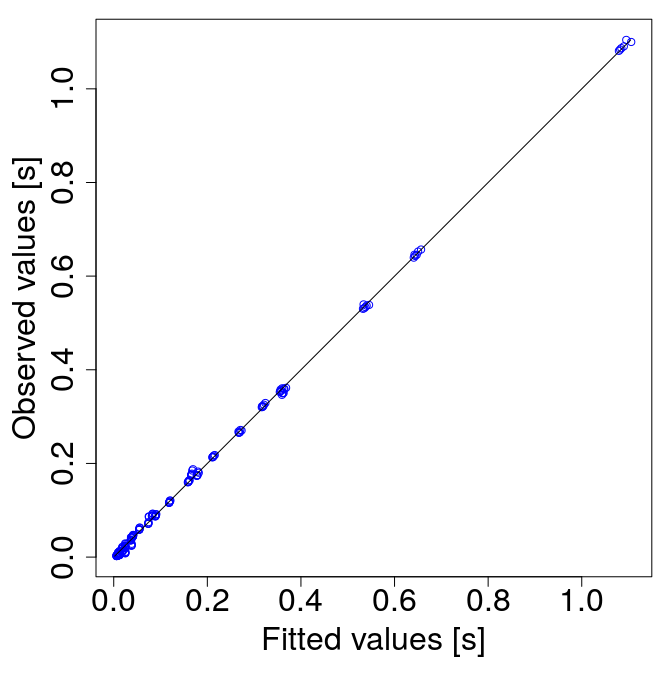
\includegraphics[scale=0.22]{figures/actionK-HTFETI-FvO.png}
%\end{minipage}
%}
\caption{Action of $K$ in HTFETI}
\label{fig:actionK-HTFETI}
\end{figure}

\paragraph{The remaining partial models} describe:  %listed in the Appendix \ref{sec:partialModels}. Those models describe 
assembling ($t_{K|asm}$), factorization ($t_{K|fact}$) and action ($t_{K|act|T}$,$t_{K|act|HT}$) of the stiffness matrices $K_i$ for all subdomains; assembling ($t_{Dir|asm}$) and action ($t_{Dir|act}$) of Dirichlet preconditioner for all subdomains; action of the Lumped preconditioner $t_{Lump|act}$ for all subdomains, assembling ($t_{GG^T|asm|T}$,$t_{GG^T|asm|HT}$) and action ($t_{GG^T|act|T}$, $t_{GG^T|act|HT}$) of the coarse problem $GG^T$, assembling the HTFETI objects ($t_{S\alpha|asm}$, $t_{F_0|asm}$). The $_{|T}$ stands for  Total FETI and $_{|HT}$ stands for HTFETI. 

\subsection{Full Model}
The final model for the TFETI method without Dirichlet preconditioner is given by the following formula
% \begin{equation}
% \begin{aligned}
% &\verb!time ~ timeAsmK + timeFactK + timeAsmGGTT!\\
% &\verb!       + iterNum*(timeActKT + timeActGGTT + timeActPrec),!
% \end{aligned}
% \label{eq:finalTFETI}
% \end{equation}

\begin{equation}
\begin{aligned}
t_e \approx\; &t_{K|asm} + t_{K|fact} + t_{GG^T|asm|T}\\ &+ iter \cdot (t_{K|act|T} + t_{GG^T|act|T} + t_{Prec|act}),
\end{aligned}
\label{eq:finalTFETI}
\end{equation}
where $t_e$ is the estimated run-time of ESPRESO, $iter$ is the estimated number of PPCG iterations  and $t_{Prec|act}$ equals $t_{Lump|act} + t_{GG^T|act|T}$ if Lumped preconditioner is used or 0 if there is no preconditioner.


When using Dirichlet preconditioner which requires extra preprocessing time the formula must be modified to

\begin{equation}
\begin{aligned}
t_e \approx\;  &t_{K|asm} + t_{K|fact} +  t_{GG^T|asm|T} +  t_{Dir|asm}\\ &+ iter\cdot(t_{K|act} + 2t_{GG^T|act|T} + t_{Dir|act})  
\end{aligned}
\label{eq:finalTFETIDirichlet}
\end{equation}
For HTFETI method both formulas remain very similar, only $t_{GG^T|asm|T}$, t$_{GG^T|act|T}$ and $t_{K|act|T}$ will be replaced with $t_{GG^T|asm|HT}$, t$_{GG^T|act|HT}$, $t_{K|act|HT}$. In case of the HTFETI method an extra preprocessing is also necessary $t_{F_0|asm}$, t$_{S\alpha|asm}$. 


So, the model for HTFETI without preconditioner or using Lumped preconditioner
will be modified as

\begin{equation}
\begin{aligned}
t_e \approx\; &t_{F|asm} + t_{S_\alpha|asm} + t_{K|asm} + t_{K|fact} + t_{GG^T|asm|HT} \\
&+ iter \cdot (t_{K|act|HT} + t_{GG^T|act|HT} + t_{Prec|act})
\end{aligned}
\label{eq:finalHTFETI}
\end{equation}
and the model for HTFETI with Dirichlet preconditioner as

\begin{equation}
\begin{aligned}
t_e \approx\; &t_{F|asm} + t_{S_\alpha|asm} + t_{K|asm} + t_{K|fact} + t_{GG^T|asm|HT}  + t_{Dir|asm}\\
&+ iter \cdot (t_{K|act|HT} + 2t_{GG^T|act|HT} + t_{Dir|act})
\end{aligned}
\label{eq:finalHTFETIDirichlet}
\end{equation}


\section{Model Validation}
The final model was validated using RMSE\cite{rmse}, sMAPE\cite{smape} and finally
by the simple comparison of the difference between measured run-time with estimated 
optimal settings and the manually found optimal run-time.

We can see the whole fit of the final TFETI and HTFETI model in Fig. \ref{fig:finalTFETIModel} and \ref{fig:finalHTFETIModel}, respectively.

\begin{figure}[htb]
\centering
\begin{minipage}{0.3\textwidth}
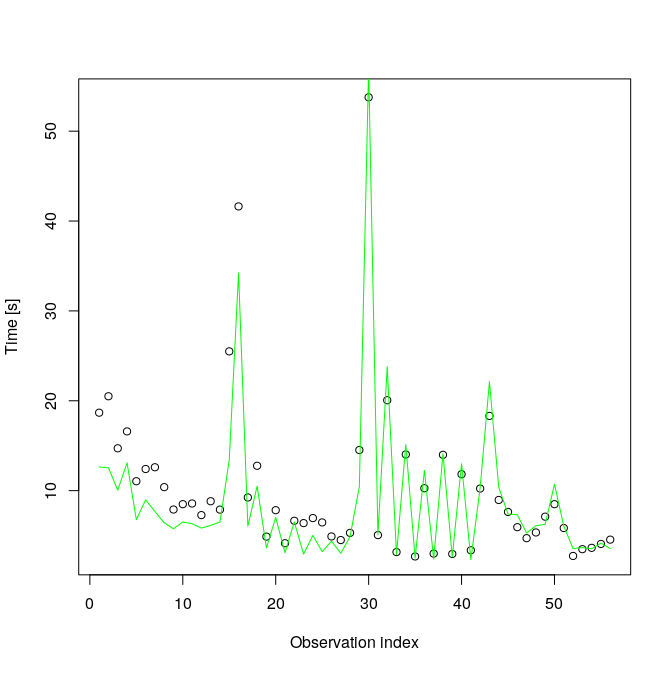
\includegraphics[width=\textwidth]{figures/tfeti-none.png}
\end{minipage}
\begin{minipage}{0.3\textwidth}
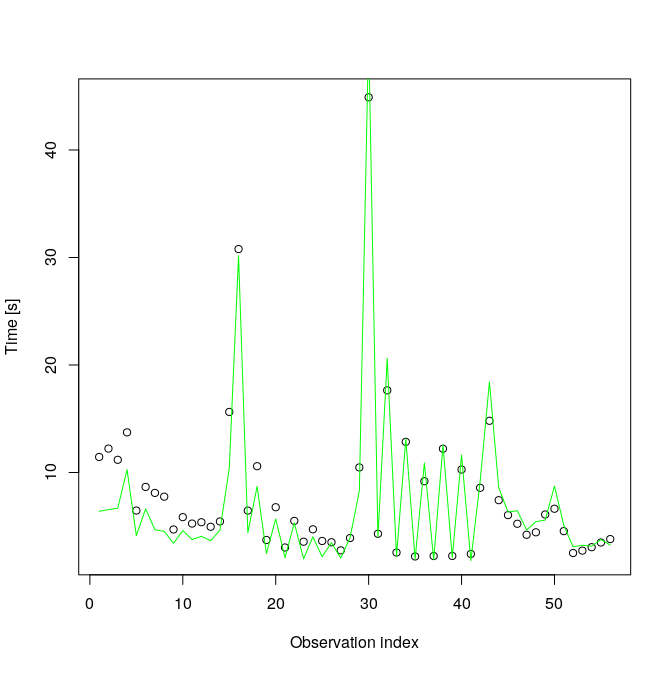
\includegraphics[width=\textwidth]{figures/tfeti-lumped.png}
\end{minipage}
\begin{minipage}{0.3\textwidth}
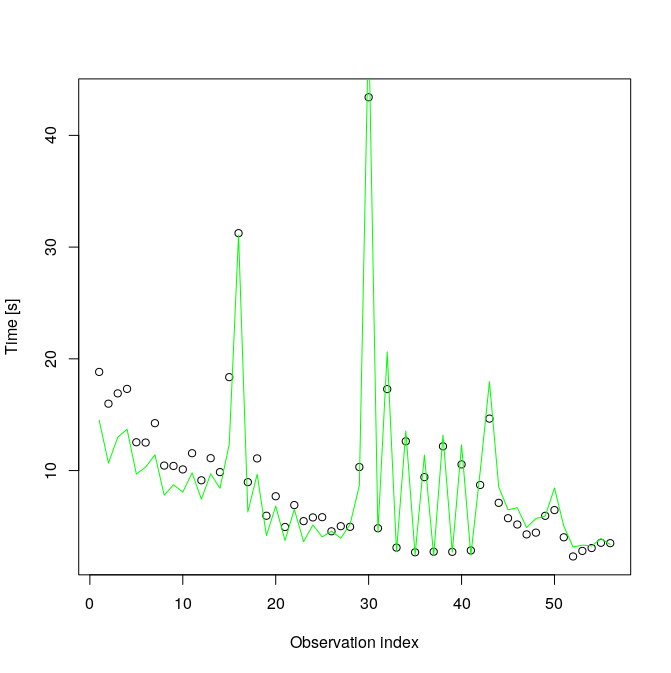
\includegraphics[width=\textwidth]{figures/tfeti-dirichlet.png}
\end{minipage}
\caption{Total FETI model fit with: no preconditioner (left), Lumped precondition (middle) and Dirichlet preconditioner (right).}
\label{fig:finalTFETIModel}
\end{figure}

The estimations of the optimal settings and their comparison with real optima can be seen in the Tab. \ref{tab:finalModelTest}, where \textit{Predicted time} is the 
minimal run-time estimated by the model together with the corresponding \textit{Predicted settings}. \textit{Measured time from predicted settings} is the 
manually measured run-time using the predicted settings from the model estimation. 
\textit{Optimal time} is then the manually found optima and \textit{Optimal settings} 
are the corresponding settings to the optimal time. Finally, \textit{Prediction error} is the difference between the measured time from predicted settings and the 
optimal time, i.e. the difference users would get if they were using the model for their computations.

\begin{table}[!htb]
\centering
\begin{tabular}{lcccccc}
\multicolumn{1}{c}{} & \multicolumn{6}{c}{\textbf{1728000 DOFs}} \\ \cline{2-7} 
\multicolumn{1}{l|}{} & \multicolumn{3}{c}{\textbf{TFETI}} & \multicolumn{3}{c|}{\textbf{HTFETI}} \\ \hline
\multicolumn{1}{|r|}{\textbf{Preconditioner}} & \multicolumn{1}{c|}{\textbf{None}} & \multicolumn{1}{c|}{\textbf{Lumped}} & \multicolumn{1}{c|}{\textbf{Dirichlet}} & \multicolumn{1}{c|}{\textbf{None}} & \multicolumn{1}{c|}{\textbf{Lumped}} & \multicolumn{1}{c|}{\textbf{Dirichlet}} \\ \hline
\multicolumn{1}{|l|}{\begin{tabular}[c]{@{}l@{}}Predicted settings: \\ \# of compute nodes \\ \# of MPI processes per node\\ \# of Cilk threads per MPI p.\\ \# of domains per MPI rank \\ domain size {[}DOF{]}\end{tabular}} & \begin{tabular}[c]{@{}c@{}}4\\ 24\\ 1\\ 18\\ 1029\end{tabular} & \begin{tabular}[c]{@{}c@{}}4\\ 24\\ 1\\ 18\\  1029\end{tabular} & \multicolumn{1}{c|}{\begin{tabular}[c]{@{}c@{}}4\\ 8\\ 3\\ 48\\ 1029\end{tabular}} & \begin{tabular}[c]{@{}c@{}}16\\ 4\\ 6\\ 64\\ 375\end{tabular} & \begin{tabular}[c]{@{}c@{}}16\\ 24\\ 1\\ 12\\ 375\end{tabular} & \multicolumn{1}{c|}{\begin{tabular}[c]{@{}c@{}}16\\ 4\\ 6\\ 64\\ 375\end{tabular}} \\ \hline
\multicolumn{1}{|l|}{Predicted time {[}s{]}} & 2.32 & 1.8 & \multicolumn{1}{c|}{2.39} & 0.78 & 0.66 & \multicolumn{1}{c|}{0.76} \\ \hline
\multicolumn{1}{|l|}{\begin{tabular}[c]{@{}l@{}}Measured time from \\ predicted settings {[}s{]}\end{tabular}} & 3.36 & 2.42 & \multicolumn{1}{c|}{2.74} & 0.77 & 1.05 & \multicolumn{1}{c|}{0.54} \\ \hline
\multicolumn{1}{|l|}{\begin{tabular}[c]{@{}l@{}}Optimal settings:\\ \# of compute nodes \\ \# of MPI processes per node\\ \# of Cilk threads per MPI p.\\ \# of domains per MPI rank \\ domain size {[}DOF{]}\end{tabular}} & \begin{tabular}[c]{@{}c@{}}4\\ 6\\ 4\\ 64\\ 1029\end{tabular} & \begin{tabular}[c]{@{}c@{}}4\\ 6\\ 4\\ 64\\ 1029\end{tabular} & \multicolumn{1}{c|}{\begin{tabular}[c]{@{}c@{}}16\\ 4\\ 6\\ 64\\ 375\end{tabular}} & \begin{tabular}[c]{@{}c@{}}16\\ 4\\ 6\\ 64\\ 375\end{tabular} & \begin{tabular}[c]{@{}c@{}}16\\ 4\\ 6\\ 64\\ 375\end{tabular} & \multicolumn{1}{c|}{\begin{tabular}[c]{@{}c@{}}16\\ 4\\ 6\\ 64\\ 375\end{tabular}} \\ \hline
\multicolumn{1}{|l|}{Optimal time {[}s{]}} & 2.68 & 2.19 & \multicolumn{1}{c|}{2.31} & 0.77 & 0.53 & \multicolumn{1}{c|}{0.54} \\ \hline
\multicolumn{1}{|l|}{RMSE} & 3.14 & 2.13 & \multicolumn{1}{c|}{2.21} & 4 & 1.37 & \multicolumn{1}{c|}{1.49} \\ \hline
\multicolumn{1}{|l|}{sMAPE} & 0.23 & 0.23 & \multicolumn{1}{c|}{0.18} & 0.43 & 0.27 & \multicolumn{1}{c|}{0.24} \\ \hline
\multicolumn{1}{|l|}{Prediction error {[}s{]}} & 0.69 & 0.23 & \multicolumn{1}{c|}{0.42} & 0 & 0.51 & \multicolumn{1}{c|}{0} \\ \hline
\end{tabular}
\caption{Evaluation of the final model prediction quality}
\label{tab:finalModelTest}
\end{table}

\begin{figure}[htb]
\centering
\begin{minipage}{0.3\textwidth}
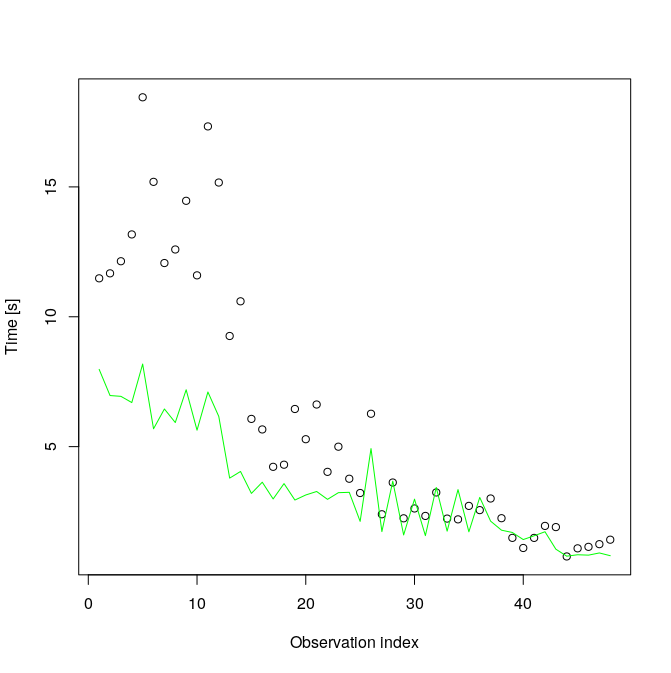
\includegraphics[width=\textwidth]{figures/htfeti-none.png}
\end{minipage}
\begin{minipage}{0.3\textwidth}
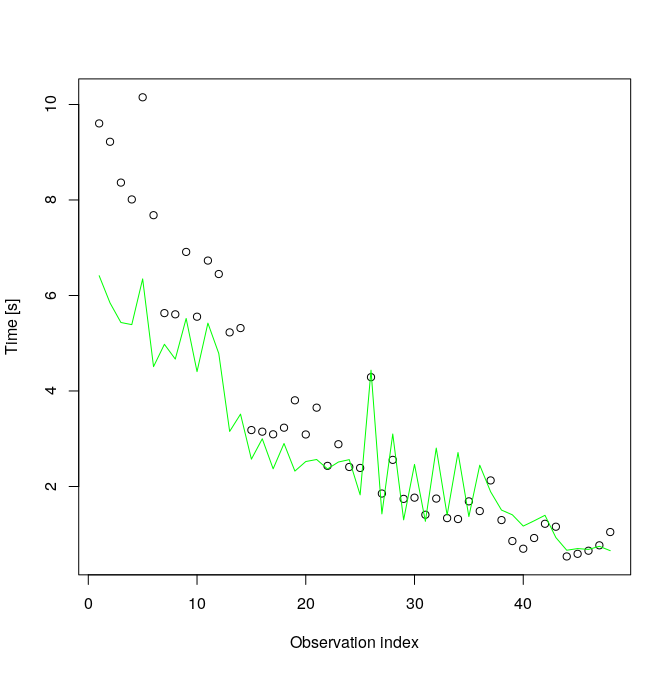
\includegraphics[width=\textwidth]{figures/htfeti-lumped.png}
\end{minipage}
\begin{minipage}{0.3\textwidth}
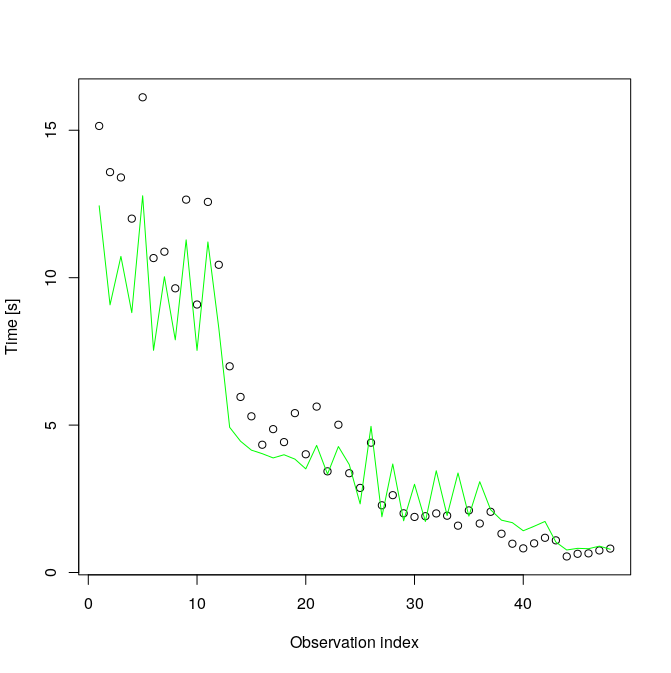
\includegraphics[width=\textwidth]{figures/htfeti-dirichlet.png}
\end{minipage}
\caption{Hybrid Total FETI model fit with: no preconditioner (left), Lumped precondition (middle) and Dirichlet preconditioner (right).}
\label{fig:finalHTFETIModel}
\end{figure}
\section{Conclusion}
Our approach significantly simplifies the optimal usage of the FETI solvers in ESPRESO library 
and can provided significant savings in orders of magnitude for both runtime as well as energy consumption for inexperienced users. 
The final model as implemented requires only following input parameters provided by user: 

\begin{itemize}
\item total problem size,
\item selected FETI method, 
\item selected preconditioner, 
\item estimated number of CG iterations (used to estimate the significance of the preprocessing routines).
\end{itemize}

while it returns the estimated solver run-time with the corresponding optimal 
decomposition, parallelization settings of the solver.

The number of CG iteration can not be predicted by our model so we left it as the user input.  
User can simply perform a single test-runs,  which will give them the approximate information 
about the number of iterations. 

The estimated run-time was predicted with deviation lesser than 1\,s, given the 
measured minimal time, as can be seen in the Tab. \ref{tab:finalModelTest}. 
This is an acceptable precision, as with the least suitable settings the
run-time can be more than 20 times (i.e. more than 50\,s in this case) slower  
as the the optimal one.


{\renewcommand{\markboth}[2]{}%
\printbibliography[heading=bibintoc]}
%\bibliographystyle{splncs03}
%\bibliography{References}

\appendix
\section{Basic Description of the R-syntax}
\label{sec:r}
The modeling itself was performed in R language (see \cite{rDocs}), which is
a specialized programming language for statistical computations. Because the R-syntax is
capable of containing the information about polynomials and term interaction in a 
relatively compact format this syntax is used to describe the models in this thesis.


The input variables such as the number of nodes, number of MPI processes (i.e. number of clusters) per 
node, number of domains per cluster and number of DOF per node were denoted as 
\texttt{nnodes}, \texttt{nprocs}, \texttt{ndoms} and \texttt{nDOF}, respectively.


\paragraph*{Fitting a model} was accomplished with the function \texttt{glm()}\footnote{\url{https://stat.ethz.ch/R-manual/R-devel/library/stats/html/glm.html}}.
% , which performs the Fisher scoring algorithm  to fit the generalized linear model. The example can be seen in Lst. \ref{lst:glmExample}.


% \begin{lstlisting}[language=R,
% 				   caption=Fitting the function using generalized linear regression in R,
%                    label=lst:glmExample,
%                    linewidth=8cm]
% fit1 <- glm(formula=time ~ (poly(I(1/nprocs), 2) 
%                             + poly(ndoms, 2) 
%                             + poly(nDOF, 2))^3,
%             data=dataFact,
%             family=gaussian(link="log"))
% \end{lstlisting}


\paragraph*{\textit{Formula}} is described by a special syntax whose brief overview follows. Several examples can be seen in  Tab. \ref{tab:rFormulaSyntax}.

\begin{itemize}
	\item[]$\sim$ denotes "a dependency". If used in GLM, then it describes the response dependent on
	a predictor - i.e. we can substitute it with $=$ in a mathematical notation.
	\item[]$\left(x + y\right)\string^\,n$ describes main effects and all interaction up to the 
	n-th order of the listed variables.
	\item[]$I\left( \cdots \right)$ describes the environment with numeric operations, e.g. $I\left( x\string^2 \right) = x^2$, $I\left( log\left(x\right) \right) = \ln x$ etc.
	\item[]$poly\left(x, n\right)$ describes an orthogonal polynomial of the variable $x$ up to the n-th
	order.
	\item[]$poly\left(x, n, raw=T\right)$ describes an ordinary polynomial of the variable $x$ up to the 
	n-th order.
\end{itemize}


An orthogonal polynomial is internally computed as a model matrix of an ordinary polynomial and then its
columns are adjusted to be orthogonal to all the previous ones. The first advantage of the orthogonality 
is, that coefficients remain the same while adding new ones, i.e. $\beta_0$ and $\beta_1$ in the 
polynomial $\beta_0 + \beta_1x$ will not change their values after adding $\beta_2x^2$ etc.


% We can show it on a simple example, given by the Lst. \ref{lst:polyExampleM}.


% \begin{lstlisting}[language=R,
% 				   caption=The effect of adding a new term into the orthogonal polynomial in R,
%                    label=lst:polyExampleM]
% m <- lm(dist ~ poly(speed, 1), data = cars, x=T)
% m1 <- lm(dist ~ poly(speed, 2), data = cars, x=T)
% \end{lstlisting}


% The coefficients of the model $m$, obtained by a \texttt{summary()} function look like this:

% \begin{figure}[H]
% \centering
% \begin{minipage}{0.45\textwidth}
% \centering
% \begin{BVerbatim}
%                Estimate
% (Intercept)      42.980     
% poly(speed, 1)  145.552     
% \end{BVerbatim}
% \end{minipage}
% \begin{minipage}{0.45\textwidth}
% \centering
% \begin{BVerbatim}
%                 Estimate
% (Intercept)       42.980
% poly(speed, 2)1  145.552
% poly(speed, 2)2   22.996
% \end{BVerbatim}
% \end{minipage}
% \end{figure}


% And we can see, that after adding another term into the polynomial of the $speed$ variable (see model 
% $m1$ in listing \ref{lst:polyExampleM}), the first two coefficients did not change at all.


The second advantage of the orthogonal polynomials is, that while the previous terms keep their 
coefficients, the new terms add only new "effects" to the model. So if the new term is not significantly
contributing to the model, it can be easily detected with Wald test with $H_0: \beta_i = 0$, $\beta_i$ being the i-th coefficient of a linear predictor in a generalized linear regression.

\begin{table}[hbt]
\centering
\begin{tabular}{lr}
\hline
\textbf{R formula} & \textbf{Meaning} \\ 
\hline
\texttt{y $\sim$ x + z} & $y = \beta_0 + \beta_1x  + \beta_2z$ \\
\texttt{x + z + x:z} & $\beta_0 + \beta_1x + \beta_2z + \beta_3 x z$ \\
\texttt{(x + y + z)\string^3} & $\beta_0 + \beta_1x + \beta_2y + \beta_3z + \beta_4 x y + 
\beta_5 x z + \beta_6 y z + \beta_7 x yz$ \\
\texttt{poly(x, 2, raw=T)} & $\beta_0 + \beta_1x + \beta_2 x^2$ \\
\texttt{I(1/x)} & $\frac{1}{x}$ \\
\hline
\end{tabular}
\caption{Examples of R formula syntax}
\label{tab:rFormulaSyntax}
\end{table}


When using ordinary polynomials, coefficients of the previous terms change with every new term added 
to the polynomial. Therefore the contribution of every single new term can not be detected so easily. This 
could result in all the terms in the ordinary polynomial being detected as non-significant by Wald test, 
despite the fact, that only its last term does not contribute to the model.


The main advantage of the ordinary polynomials over the orthogonal ones is their easy interpretation,
as can be seen in the Tab. \ref{tab:rFormulaSyntax}. So, the orthogonal polynomials were mostly 
used in this thesis during the process of creating models and when the model was well-fitting and simple 
enough, they were replaced with ordinary ones, to make formulas easy to understand and easy to write 
down, if needed. 

\section{List of Partial Models}
\label{sec:partialModels}

\begin{align}
&\begin{aligned}
t_{K|act|T} \sim\; &\mathrm{poly(I(1/nprocs), 3, raw=T) + poly(ndoms, 3, raw=T)}\\
&+ \mathrm{poly(nDOF, 3, raw=T)}\\
&+ \mathrm{I(1/nprocs):poly(nDOF, 2, raw=T)}
\end{aligned}\\[10pt]
&\begin{aligned}
t_{Dir|act} \sim\; &\mathrm{poly(I(1/nprocs), 3, raw=T) + poly(nDOF, 3, raw=T)}\\
&+ \mathrm{poly(ndoms, 3, raw=T)}
\end{aligned}\\[10pt]
&\begin{aligned}
t_{Lump_|act} \sim\; &\mathrm{poly(I(1/nprocs), 3, raw=T)}\\
&+ \mathrm{poly(ndoms, 3, raw=T) + poly(nDOF, 3, raw=T)}\\
&+ \mathrm{I(1/nprocs):nDOF}
\end{aligned}\\[10pt]
&\begin{aligned}
t_{Dir|asm} \sim\; &\mathrm{poly(I(1/nprocs), 2, raw=T) + poly(nDOF, 4, raw=T)}\\
&+ \mathrm{poly(ndoms, 3, raw=T)}
\end{aligned}\\[10pt]
&\begin{aligned}
t_{K|asm} \sim\; &\mathrm{poly(I(1/nprocs), 2 ,raw=T) + poly(nDOF, 3, raw=T)}\\
&+ \mathrm{poly(ndoms, 3, raw=T)}\\
&+ \mathrm{I(1/nprocs):poly(ndoms, 2, raw=T)}
\end{aligned}\\[10pt]
&\begin{aligned}
t_{F|asm}  \sim\; &\mathrm{poly(I(1/nprocs), 3, raw=T)}\\
&+ \mathrm{poly(ndoms, 3, raw=T)}\\
&+ \mathrm{poly(nDOF, 3, raw=T)}
\end{aligned}\\[10pt]
&\begin{aligned}
t_{K|fact} \sim\; &\mathrm{poly(I(1/nprocs), 2) + poly(nDOF, 3)}\\
&+ \mathrm{poly(ndoms, 3) + I(1/nprocs):poly(nDOF, 3)}
\end{aligned}\\[10pt]
&\begin{aligned}
t_{GG^T|asm|HT} \sim\; &\mathrm{poly(I(1/nprocs), 3, raw=T)}\\
&+ \mathrm{poly(nnodes, 3, raw=T) + poly(nDOF, 3, raw=T)}\\
&+ \mathrm{poly(ndoms, 3, raw=T)}\\
&+ \mathrm{poly(I(1/nprocs), 2, raw=T):ndoms + ndoms:nDOF}\\
&+ \mathrm{I(1/nprocs\,\widehat{}\,2):nnodes}
\end{aligned}\\[10pt]
&\begin{aligned}
t_{GG^T|asm|T} \sim\; &\mathrm{poly(nnodes, 3, raw=T) + poly(ndoms, 2, raw=T)}\\
&+ \mathrm{poly(nDOF, 3, raw=T)}\\
&+ \mathrm{poly(I(1/nprocs), 3, raw=T)}\\
&+ \mathrm{poly(nnodes, 3, raw=T):poly(nDOF, 3, raw=T)}\\
&+ \mathrm{poly(nDOF, 3, raw=T):poly(I(1/nprocs), 3, raw=T)}\\
&+ \mathrm{poly(nnodes, 3, raw=T):poly(I(1/nprocs), 3, raw=T)}
\end{aligned}\\[10pt]
&\begin{aligned}
t_{GG^T\: 1|asm|T} \sim\; &\mathrm{nnodes + poly(I(log(2*nnodes)), 3, raw=T)}\\
&+ \mathrm{poly(ndoms, 2, raw=T)}\\
&+ \mathrm{poly(nDOF, 3, raw=T)}\\
&+ \mathrm{I(log(2*nnodes)\,\widehat{}\,3):poly(nDOF, 2, raw=T)}
\end{aligned}\\[10pt]
&\begin{aligned}
t_{GG^T\: 2|asm|T} \sim\; &\mathrm{poly(nnodes, 3, raw=T) + poly(ndoms, 2, raw=T)}\\
&+ \mathrm{poly(nDOF, 3, raw=T)}\\
&+ \mathrm{poly(nnodes, 2, raw=T):poly(nDOF, 2, raw=T)}
\end{aligned}\\[10pt]
&\begin{aligned}
t_{GG^T|act|HT} \sim\; &\mathrm{poly(nDOF, 3, raw=T)+ I(ndoms\,\widehat{}\,2)}\\
&+ \mathrm{(poly(I(1/nprocs), 2, raw=T)}\\
&+ \mathrm{poly(nnodes, 2, raw=T))\,\widehat{}\,2}\\
&+ \mathrm{I(1/nprocs):nDOF}\\
&+ \mathrm{(poly(nnodes, 2, raw=T) + ndoms)\,\widehat{}\,2}\\
&+ \mathrm{nnodes:nDOF + nDOF:ndoms}
\end{aligned}\\[10pt]
&\begin{aligned}
t_{GG^T|act|T} \sim\; &\mathrm{poly(nnodes, 3, raw=T) + poly(I(1/nprocs), 3, raw=T)}\\
&+ \mathrm{poly(ndoms, 3, raw=T) + poly(nDOF, 2, raw=T)}\\
&+ \mathrm{poly(nnodes, 3, raw=T):nDOF + nnodes:ndoms}
\end{aligned}\\[10pt]
&\begin{aligned}
t_{S_\alpha|asm} \sim\; &\mathrm{nDOF + poly(I(1/nprocs), 3, raw=T)}\\
&+ \mathrm{poly(ndoms, 2, raw=T)}\\
&+ \mathrm{poly(nDOF, 3, raw=T):poly(I(1/nprocs), 3, raw=T)}
\end{aligned}
\end{align}





\end{document}
